\documentclass[a4paper, 10pt]{article}
%\usepackage{fontspec}
%\setmainfont{Lato}
\usepackage{pgf}
\usepackage{eurosym}
\usepackage{graphicx}
\usepackage{wasysym}
\usepackage{hyperref}
\usepackage{listings}
\usepackage{pxfonts}
\usepackage{verbatim}
\usepackage{color}
\usepackage{xcolor}
\usepackage{wrapfig}
\usepackage{enumitem}
\usepackage{booktabs}
\usepackage{gensymb}
\usepackage{tabularx}
\usepackage{currfile}

\hypersetup{
    bookmarks=true,         % show bookmarks bar?
    unicode=true,          % non-Latin characters in Acrobat’s bookmarks
    pdftoolbar=true,        % show Acrobat’s toolbar?
    pdfmenubar=true,        % show Acrobat’s menu?
    pdffitwindow=true,     % window fit to page when opened
    pdftitle={Assessments},    % title
    pdfauthor={Paul Vesey},     % author
    pdfsubject={Advanced Graphics Assignment },   % subject of the document
    pdfcreator={},   % creator of the document
    pdfproducer={xelatex}, % producer of the document
    pdfkeywords={'Graphics' }, % list of keywords
    pdfnewwindow=true,      % links in new PDF window
    colorlinks=true,       % false: boxed links; true: colored links
    linkcolor=violet,          % color of internal links (change box color with linkbordercolor)
    citecolor=magenta,        % color of links to bibliography
    filecolor=red,      % color of file links
    urlcolor=blue           % color of external links
}

\setlength\parindent{0pt}
\begin{document}

\lstset{language=HTML,
				basicstyle=\small,
				breaklines=true,
        numbers=left,
        numberstyle=\tiny,
        showstringspaces=false,
        aboveskip=-20pt,
        frame=leftline
        }
				
\begin{table}%
	\begin{minipage}{0.4\textwidth}%
			
\includegraphics[width=1\textwidth]{./img/LITlogo.jpg}
	\end{minipage}
	\qquad
	\centering
	\parbox{0.4\textwidth}{
		\begin{large}			
			\begin{tabular}{| r | l |} \hline
				Subject: & \textbf{Advanced Graphics}\\
								 & \textbf{\& Visualisation}\\
				Course: & \textbf{Interior Design Y3}\\
				Session: & \textbf{Autumn 2020}\\
				Lecturer: & \textbf{Paul Vesey \footnotesize{BEng, MIE, HDip}}\\
				Filename: & \footnotesize{\currfilename}\\
				\hline
			\end{tabular}
		\end{large}			
	}
\end{table}
\vspace{0.25cm}	

%     _            _                                  _     _  _   
%    / \   ___ ___(_) __ _ _ __  _ __ ___   ___ _ __ | |_  | || |  
%   / _ \ / __/ __| |/ _` | '_ \| '_ ` _ \ / _ \ '_ \| __| | || |_ 
%  / ___ \\__ \__ \ | (_| | | | | | | | | |  __/ | | | |_  |__   _|
% /_/   \_\___/___/_|\__, |_| |_|_| |_| |_|\___|_| |_|\__|    |_|  
%                    |___/                                         

\newpage
\setcounter{page}{1}
\begin{center}
	\begin{figure}[ht]
		\centering
		
\includegraphics[width = 6cm]{img/LITlogo.jpg}
		\label{fig:logoa4}
	\end{figure}
	\Large\textbf{Practical 4 - }\\
	\large\textbf{BA in Interior Design \& Technology}
\end{center}

In this assignment you are going to create a table in 3DS, complete with table cloth.  Your final image should comprise complete, set table situated in an appropriate location.  You are permitted to obtain crockery and cutlery from \href{http://www.turbosquid.com/}{http://www.turbosquid.com/}.

\\
\begin{figure}[h]
	\centering
		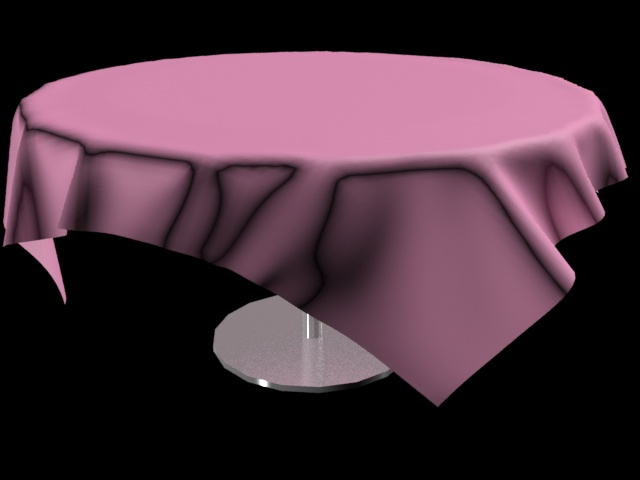
\includegraphics[width = 10cm]{img/p4Table.jpg}
	\caption{3DS Table Cloth}
	\label{fig:p4Table}
\end{figure}


\end{document}